\documentclass{article}
\usepackage{listings}
\usepackage{xcolor}
\usepackage{amsmath}
\usepackage{blindtext}
\usepackage{amssymb}
\usepackage{graphicx}
\usepackage{hyperref}
\usepackage{enumitem}
\usepackage[a4paper, margin=1in]{geometry}
\usepackage{minted}

\renewcommand{\itemautorefname}{Step}
\renewcommand{\sectionautorefname}{Section}

\title{Master Minds: The Report}
\author{
	Xinhao Su\\
	\texttt{xs2413}
	\and
	David Xu\\
	\texttt{dx2199}
}
\begin{document}
\maketitle
\section{Problem Overview}
Master Mind is a classic codebreaking game first played in 1970. Gameplay goes as follows:
\begin{enumerate}
	\item The ``codemaker'' picks four pegs and places them in order. This is the ``solution code''. Each peg can be one of six different colors and colors can be repeated between pegs.
	\item The ``codebreaker'' then has 8 turns to guess this code. On each turn:
	\begin {enumerate}
		\item The codebreaker makes a guess of the code (four pegs in order, each having one of the six colors).
		\item The codemaker responds with feedback using some number of black and white pegs. Each black peg means a peg of the guess is both the right color and in the right position. Each white peg means a peg of the guess is the right color but in the wrong position.
		\item Using this information, the codebreaker can formulate his/her next guess.
	\end{enumerate}
	\item The game ends after the code has been guessed (the codebreaker wins) or eight incorrect guesses have been made (the codemaker wins), whichever occurs first.
\end{enumerate}

A photo of a physical game board is shown below, albeit with slightly different colors.
\begin{figure}[h]
	\centering
	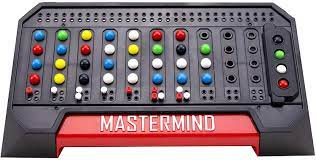
\includegraphics{mm.jpeg}
\end{figure}


\section{Formal Definition}
This game can be formalized as The Mastermind Problem. Given a set of guesses and their corresponding feedback, can we determine what solutions code(s) would produce such behavior? This is effectively a multi-dimensional search problem which has been proven to be NP-Complete\footnote{Stuckman, J., \& Zhang, G. Q. (2005). Mastermind is NP-complete. \textit{arXiv preprint cs/0512049}.}.

\section{Algorithm}
\label{sec:algorithm}
Donald Knuth proposed the ``Five-Guess Algorithm\footnote{Knuth, D. E. (1976). The computer as master mind. \textit{Journal of Recreational Mathematics, 9}(1), 1-6.}'', which was named as such because it will always determine the correct code using only at most five of the eight allowable guesses. The algorithm works as follows:
\begin{enumerate}[label=\textbf{S.\arabic*}]
	\item Generate all possible codes. Call this $S$, representing the universe of possible codes. Here, $|S| = 6^4 = 1296$.
	\item Create a set of possible solutions $P$. At the start, $P=S$.
	\item Choose an initial guess $g_0$. This can be hard-coded or randomly selected from $P$, as no information about the solution code has been obtained yet.
	\item \label{itm:algo_repeat} Play guess $g_0$ and obtain a response $r$ from the codemaker.
	\item \label{itm:algo_filter} Filter $P$ to remove all codes which could not possibly be the solution based on this response.
		\begin{itemize}
		\item For a code to possibly be the actual solution, its response to $g_0$ must also be exactly $r$.
		\end{itemize}
	\item Select the best next guess $g_1$ from $S$ using a minmax algorithm: minimize the maximum possible number of remaining codes in $P$ after this guess.
		\begin{itemize}
		\item The maximum possible number of remaining codes in $P$ after a guess $g_2$ can be calculated by determining the response of each code in $P$ to $g_2$. The response which appears with the greatest frequency is the worst case (resulting in the largest $P$ after filtering).
		\item In the case of a tie between codes, prefer a code which is still a possible solution, i.e. it is in $P$. As a final tiebreaker, select the numerically lowest code.
		\end{itemize}
	\item Repeat from \autoref{itm:algo_repeat} with guess $g_1$. Repeat until the solution is found ($|P|=1$).
\end{enumerate}

\section{Extension}
It is desirable to increase the computational difficulty of the problem so as to produce more reliable timing results. A program running over a longer amount of time will allow for recorded times to be more robust against random noise. As such, we increase the search space of the algorithm by extending the game to use $c$ colors and $h$ holes (previously, $c=6$ and $h=4$). As such, the universe of codes expands: $|S| = c^h$. For performance analyses in the remainder of this report, $c=10$ and $h=4$ are selected, resulting in $|S| = 10,000$.

\section{Sequential Implementation}
Segments of the sequential implementation are highlighted within this section. For a full code listing, see \nameref{sec:code}. Among other things, the appendix includes code allowing a human codemaker to play against the algorithm. 

\subsection{Datatypes}
\begin{minted}{haskell}
type ResponsePegs = (Int, Int) -- (#black, #white)
\end{minted}
The response providing feedback about a code is presented as a pair consisting of the number of black pegs and number of white pegs in the response.

\begin{minted}{haskell}
type Code = [Int]
\end{minted}
A code is a collection of colored pegs. Each peg is an $Int$ which correponds to a color in set $[1..c]$.

\begin{minted}{haskell}
type Possibility = (Int, Bool, Code) -- (Score, Invalid, Code)
\end{minted}
A $Possibility$ is a candidate for the next guess. The score represents the size of $P$ after this guess in the worst case. The invalid flag tracks whether the code is a possible solution (in $P$) or not. Note that finding the minimum $Possibility$ will perform the next guess selection process including tiebreakers as described in \autoref{sec:algorithm}.

\subsection{Generating a Response}
\begin{minted}{haskell}
guessResult :: Code -> Code -> ResponsePegs
guessResult ans guess = (numBlack, numWhite)
    where numBlack = length $ filter id $ zipWith (==) ans guess
          numWhite = sum (map minCodeCount $ nub guess) - numBlack
          minCodeCount v = min (count v ans) (count v guess)
          count v ls = length $ filter (==v) ls
\end{minted}
The number of black pegs ($numBlack$) can be calculated by looking for pegs in the same position with the same color. For determining the number of white pegs ($numWhite$), each color is iterated over. The minimum number of times that color appears in both codes corresponds to the number of white pegs that color will generate (e.g., three green pegs in the guess and two green pegs in the solution means two white pegs are generated). However, the number of black pegs must be subtracted from this sum (as if a peg is both the right color and in the right position, it will generate a black peg \textit{instead} of a white peg).

\subsection{Scoring a Candidate Guess}
\begin{minted}{haskell}
scoreGuess :: CodeSet -> Code -> Possibility
scoreGuess possible code = (score, not valid, code)
    where
        valid = code `elem` possible
        allResponses = map (guessResult code) possible
        score = getMaxCount allResponses
        getMaxCount xs = maximum $ map snd $ getCounts xs
        incCount o [] = [(o, 1)]
        incCount o (x@(v, c) : xs)
            | v == o = (v, c + 1) : xs
            | otherwise = x : incCount o xs
        getCounts xs = foldr incCount [] xs
\end{minted}
Given the set of remaining possibilities $P$ ($possible$) and some candidate guess $code$, the objective is to assign a score to the code representing the maximum size of $P$ after this guess in the worst case, as described in \autoref{sec:algorithm}. The $guessResult$ function is used to determine what the codemaker would respond to $g$ in the case that each potential solution was the actual solution. The $getCounts$ function is used to count how many times each response occurs. The maximum count, determined by $getMaxCount$, corresponds to the score.

\subsection{Filtering the Possible Set}
\begin{minted}{haskell}
filterCodeSet :: CodeSet -> Code -> ResponsePegs -> CodeSet
filterCodeSet set guess response =
    filter ((response ==) . guessResult guess) set
\end{minted}
Once a guess is made and a response is received from the codemaker, some of the possible solutions in $P$ can be ruled out. Specifically, solutions which produce a response to the guess different from the one received cannot be the actual solution.

\subsection{Playing the Game}
\begin{minted}{haskell}
playMastermind ::  Code -> Code -> Int -> CodeSet -> CodeSet -> IO Int
playMastermind guess solution k fullSet possibleSet = do
  putStrLn $ "Guessing: " ++ show guess
  let response@(blk, wht) = guessResult guess solution
  putStrLn $
    "Response: " ++ show blk ++ " black and "
      ++ show wht ++ " white"
  if blk == length guess then do
    putStrLn $ "Solved: " ++ show guess
    return k
  else do
    let possibleSet' = filterCodeSet possibleSet guess response
    let possibilities = map (scoreGuess possibleSet') fullSet
    let (_, _, nextGuess) = minimum possibilities
    playMastermind nextGuess solution (k + 1) fullSet possibleSet'
\end{minted}
Each turn, a guess is played by the algorithm (codebreaker) and a response received from the codemaker. If a number of black pegs equal to the number of holes is returned, the code has been found! In some cases, the algorithm may luckily guess the correct solution without having to reduce $|P|$ to $1$. Otherwise, $P$ is filtered using the response and then the universe of possible codes $S$ is searched for the best next guess.

\subsection{Performance}
It is important to keep in mind that the performance of the algorithm is dependent on both the initial guess and the solution. For example, consider the trivial case where the initial guess is equal to the solution. The algorithm will succeed without having to search $S$ at all. For this report, performance was analyzed on a 2018 MacBook Pro with 8 logical cores. The game was configured to use 10 colors and 
4 holes. A shell script was used to feed input to the program, removing the need for human interaction. Using an initial guess of $1111$ and a solution of $2613$, the algorithm succeeded in 14 seconds (note that timings are rounded to the nearest second to show proper significance, as timings vary slightly between equivalent program executions). Using a solution of $8765$ 
instead results in a 50 second execution time as shown below.
\begin{figure}[H]
	\centering
	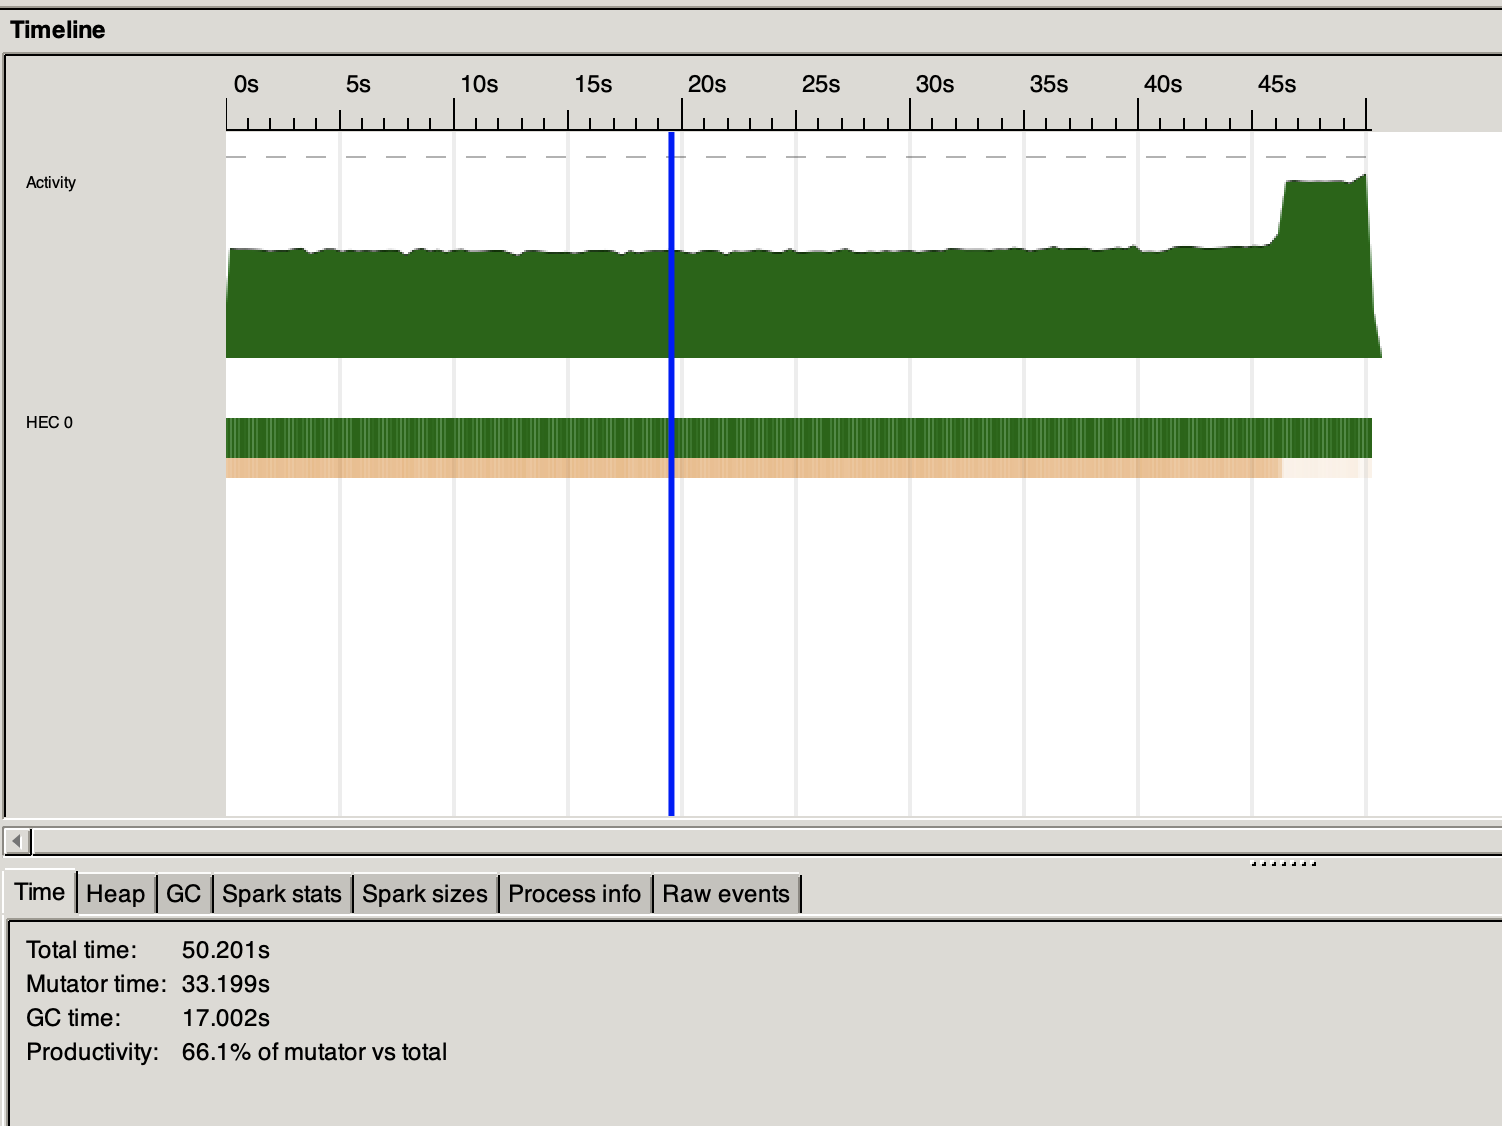
\includegraphics[width=35em]{../images/before_pl.png}
\end{figure}



\subsection{Fixing that Bump}
One may notice that towards the end of the execution above, a sudden increase in activity occurs. Analysis using Threadscope shows that this is due to stack overflows, causing the computation to stop and start again multiple times. It was determined that this was largely because of the \mintinline{haskell}{minimum} and \mintinline{haskell}{maximum} functions which are evaluated on lists of size $c^h$. This necessitates the construction and evalulation of a large redex, causing a stack overflow\footnote{https://stackoverflow.com/questions/40948153/find-min-elements-index-of-a-large-list-in-haskell}. To avoid this behavior, \mintinline{haskell}{minimum} was replaced with \mintinline{haskell}{foldl1' min}. A corresponding change was made replacing \mintinline{haskell}{maximum} with \mintinline{haskell}{foldl1' max}. Doing so alleviates the stack overflow issue (although an activity increase at the end still occurs due to computation).

\section{Parallelization}
A variety of techniques were applied to parallelize the algorithm. The most successful attempts are discussed within this section.
\subsection{Control.Monad.Par(parMap)}
\begin{minted}{haskell}
playMastermindParMap ::  Code -> Code -> Int -> CodeSet -> CodeSet -> IO Int
playMastermindParMap guess solution k fullSet possibleSet = do
  putStrLn $ "Guessing: " ++ show guess
  let response@(blk, wht) = guessResult guess solution
  putStrLn $
    "Response: " ++ show blk ++ " black and "
      ++ show wht ++ " white"
  if blk == length guess then do
    putStrLn $ "Solved: " ++ show guess
    return k
  else do
    let possibleSet' = filterCodeSet possibleSet guess response
    let possibilities = runPar $ parMap (scoreGuess possibleSet') fullSet
    let (_, _, nextGuess) = minimum possibilities
    playMastermindParMap nextGuess solution (k + 1) fullSet possibleSet'
\end{minted}
The main change here is that the $map$ over candidate guesses has been replaced with $parMap$. The result is a 21 second runtime on 8 cores, representing a performance improvement factor of 2.38.
% TODO: image from "First parMap attempt" --Solved
\begin{figure}[H]
	\centering
	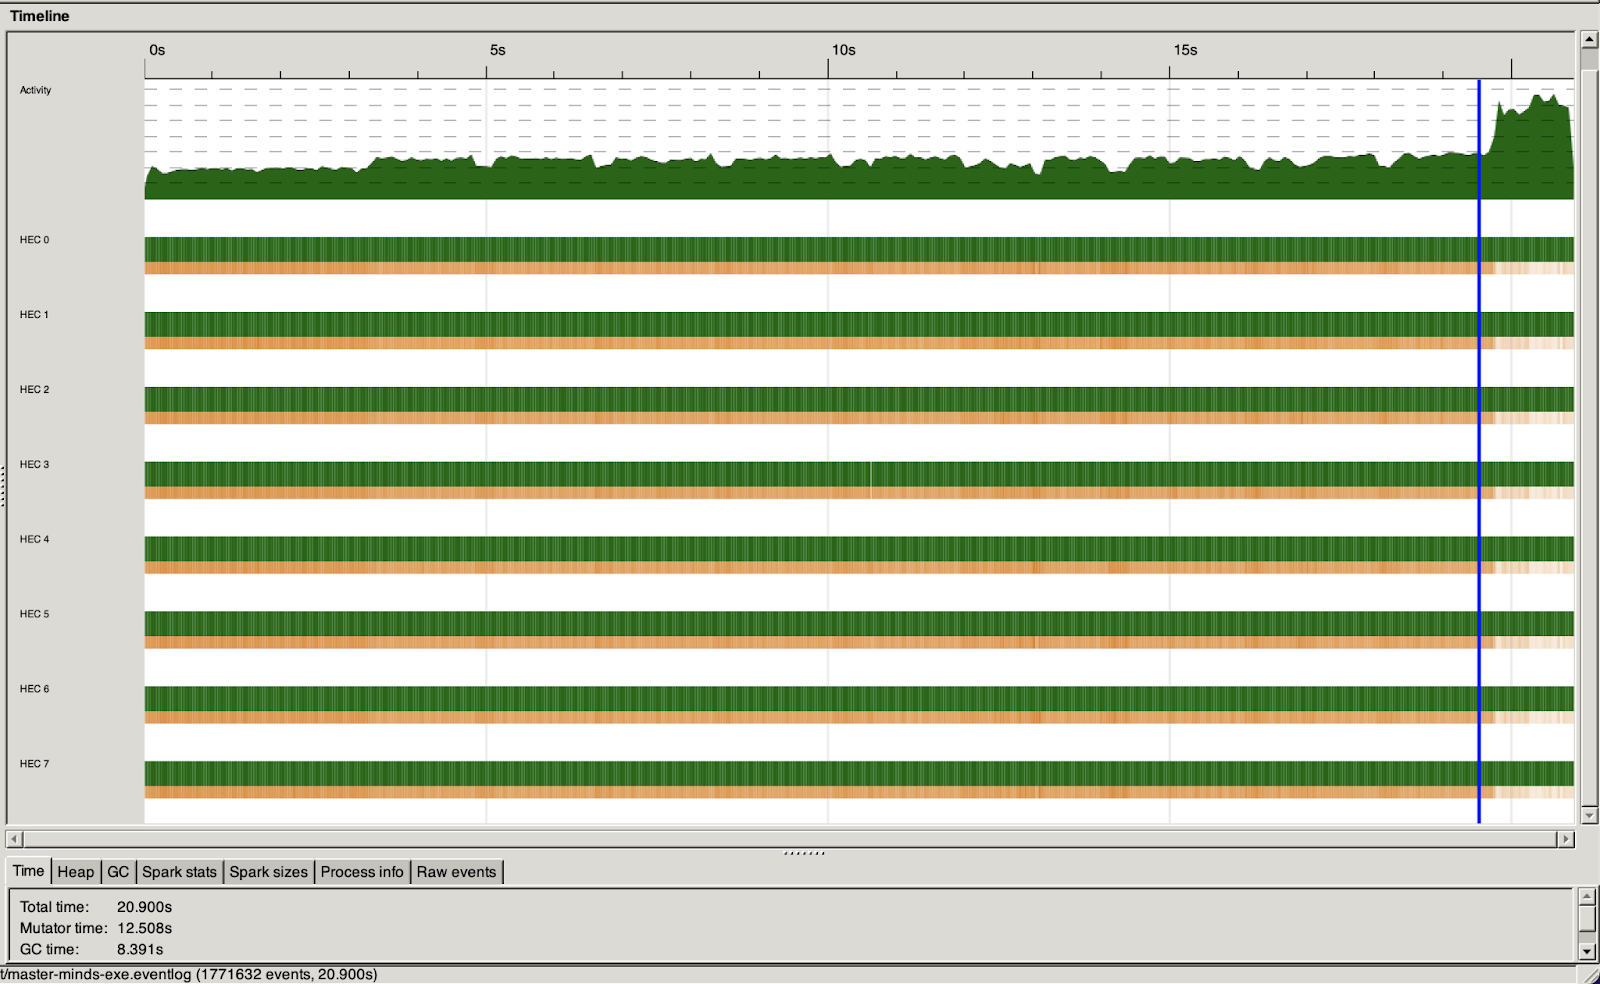
\includegraphics[width=35em]{../images/first_pm.png}
\end{figure}

Using different numbers of cores affected this performance, as shown in the graph below. As seen, increasing from 1 to 4 cores caused a significant performance improvement. Increasing past 4 cores results in minimal further improvement. This is likely because our algorithm is largely CPU-bound and the machine only has 4 physical cores mapped to 8 logical cores.
% TODO: line graph of number of cores vs. performance improvement --Solved
\begin{figure}[H]
	\centering
	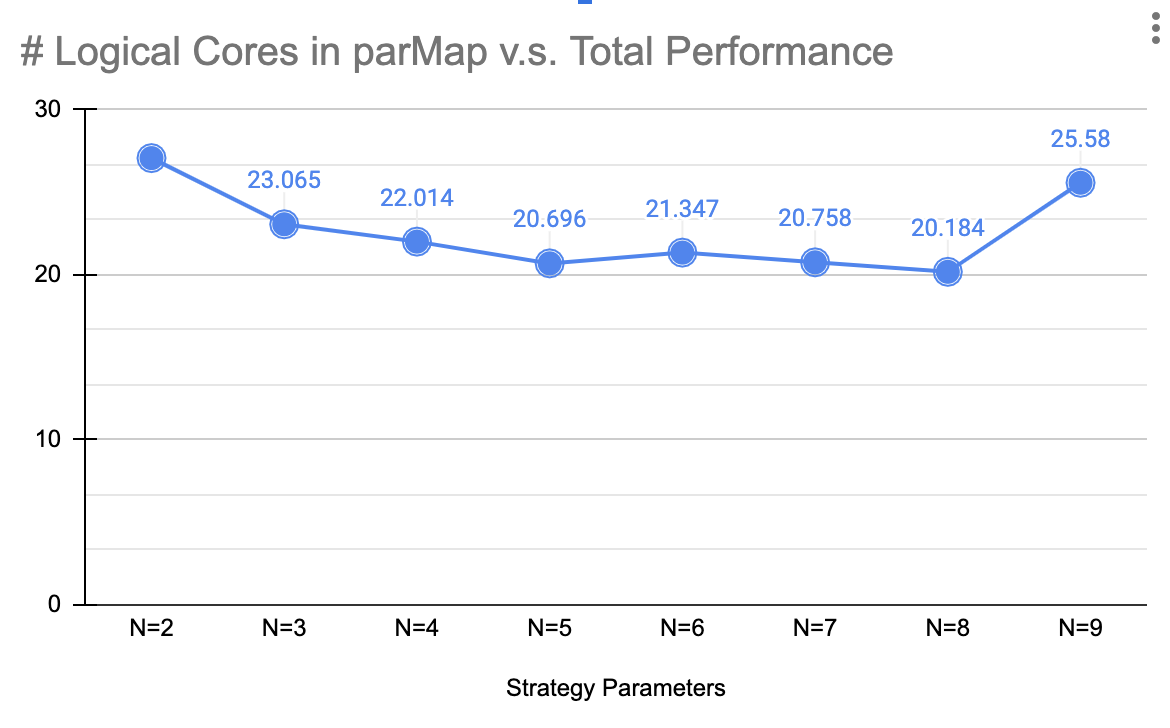
\includegraphics[width=25em]{../images/pm_line.png}
\end{figure}


At attempt was also made at using $parMap$ within the $scoreGuess$ function to parallelize the evaluation of each guess-solution pair. However, the result was extremely slow performance and a 1.2 GB event log. Evidently, too many sparks were created.
%TODO: show event log -- Solved
\begin{figure}[H]
	\centering
	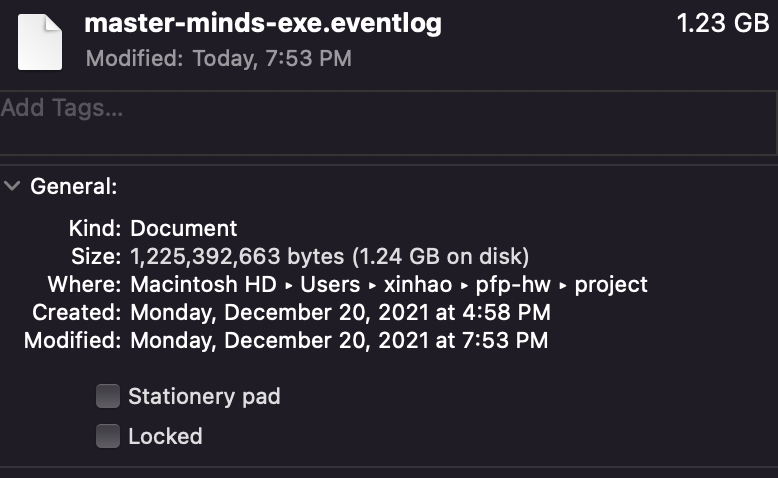
\includegraphics[width=25em]{../images/second_pm.png}
\end{figure}


%TODO: we should try to fix the bug or leave it out for the one that ran 8 CPUs but only on one of them. it's also just parMap so don't expect it to be very different. -- ?

Even with the successful parallelization above, a large number of sparks are created.

\subsection{Chunks}
Aiming to create fewer sparks, we designed a parallelization strategy which splits the candidate codes into $n$ chunks and then parallelizes computation over those chunks.
\begin{minted}{haskell}
bestFromChunk :: CodeSet -> CodeSet -> Possibility
bestFromChunk possibleSet chunk = foldl1' min $ map (scoreGuess possibleSet) chunk

-- In chunks
playMastermindChunkStrategy ::  Int -> Code -> Code -> Int -> CodeSet -> CodeSet -> IO Int
playMastermindChunkStrategy numChunks guess solution k fullSet possibleSet = do
  putStrLn $ "Guessing: " ++ show guess
  let response@(blk, wht) = guessResult guess solution
  putStrLn $
    "Response: " ++ show blk ++ " black and "
      ++ show wht ++ " white"
  if blk == length guess then do
    putStrLn $ "Solved: " ++ show guess
    return k
  else do
    let possibleSet' = filterCodeSet possibleSet guess response
    let chunks = splitToChunks numChunks fullSet -- TODO: Tune the number of chunks
    let possibilities = map (bestFromChunk possibleSet') chunks `using` parList rseq
    let (_, _, nextGuess) = foldl1' min possibilities
    playMastermindChunkStrategy numChunks nextGuess solution (k + 1) fullSet possibleSet'
\end{minted}

Notice that this strategy, aside from splitting the scoring of candidate codes into parallelized chunks, also selects the best code from each chunk. Then the best of these best-in-chunk codes is selected as the next guess. Doing so reduces the peak memory usage of the algorithm, contributing to the improved performance. Below, a Threadscope screenshot with $n=64$ chunks is shown. The run time is 17 seconds, representing a performance improvement of 2.94 times over the sequential implementation and 1.18 times over the parMap implementation running on 8 cores. Notice however that the computational load is not balanced evenly between cores.

% TODO screenshot of 64 chunks showing load balance issues -- Solved
\begin{figure}[H]
	\centering
	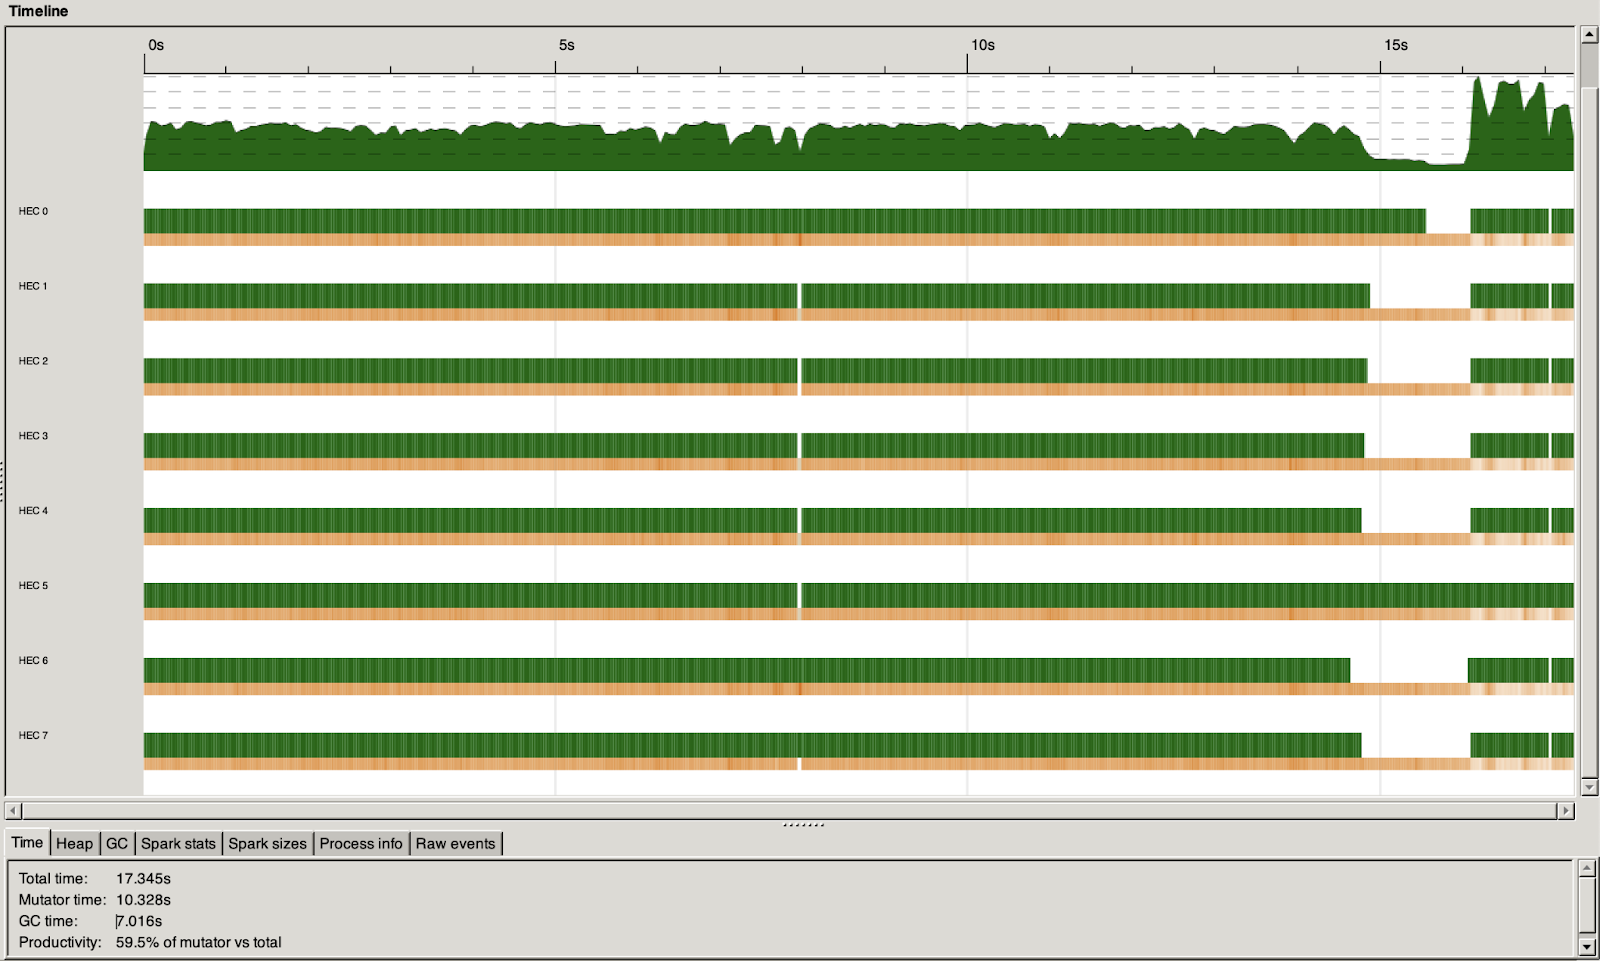
\includegraphics[width=30em]{../images/64_sc.png}
\end{figure}



Increasing the number of chunks allows for better load balancing, increasing performance. The screenshot below shows the distribution of work between cores with $n=512$ chunks. The algorithm is able to finish in 15 seconds.
% TODO screenshot of 512 chunks showing improved load balancing -- Solved
\begin{figure}[H]
	\centering
	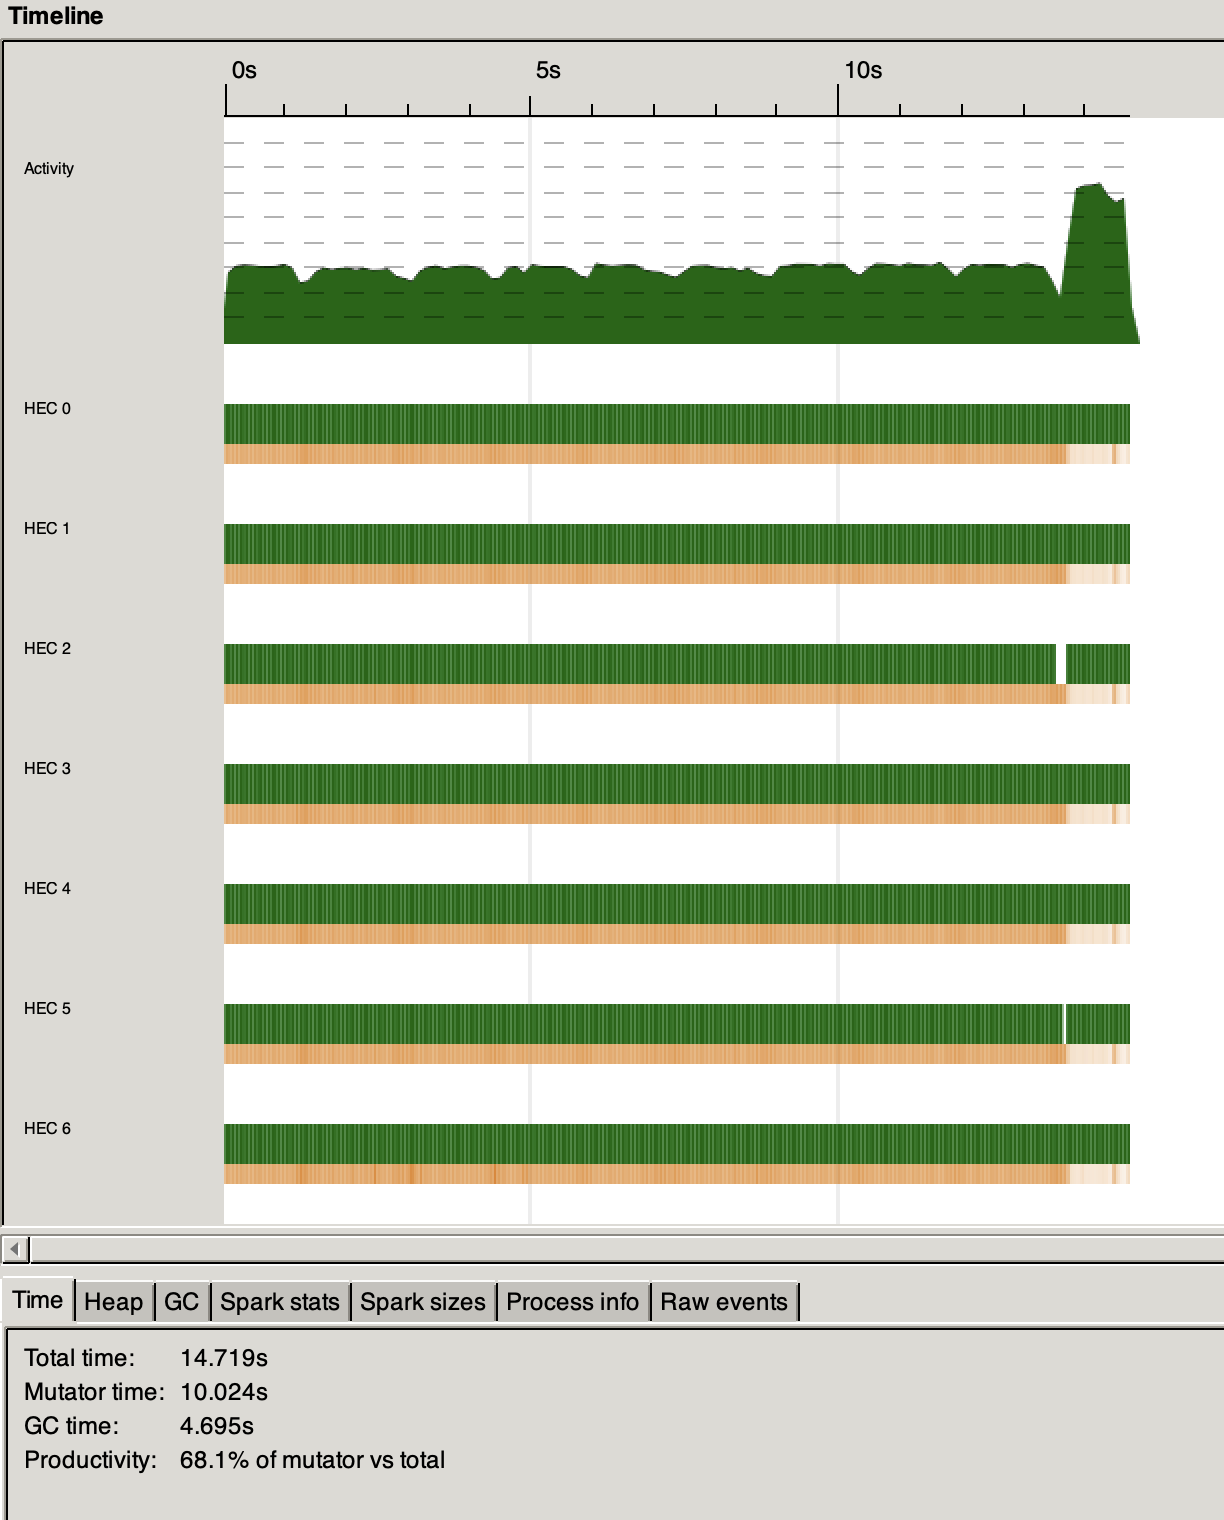
\includegraphics[width=25em]{../images/512_sc.png}
\end{figure}

Increasing $n$ past 512 results in minimal performance gains, as the load is already evenly balanced.
% TODO graph showing performance vs. number of chunks -- Solved
\begin{figure}[H]
	\centering
	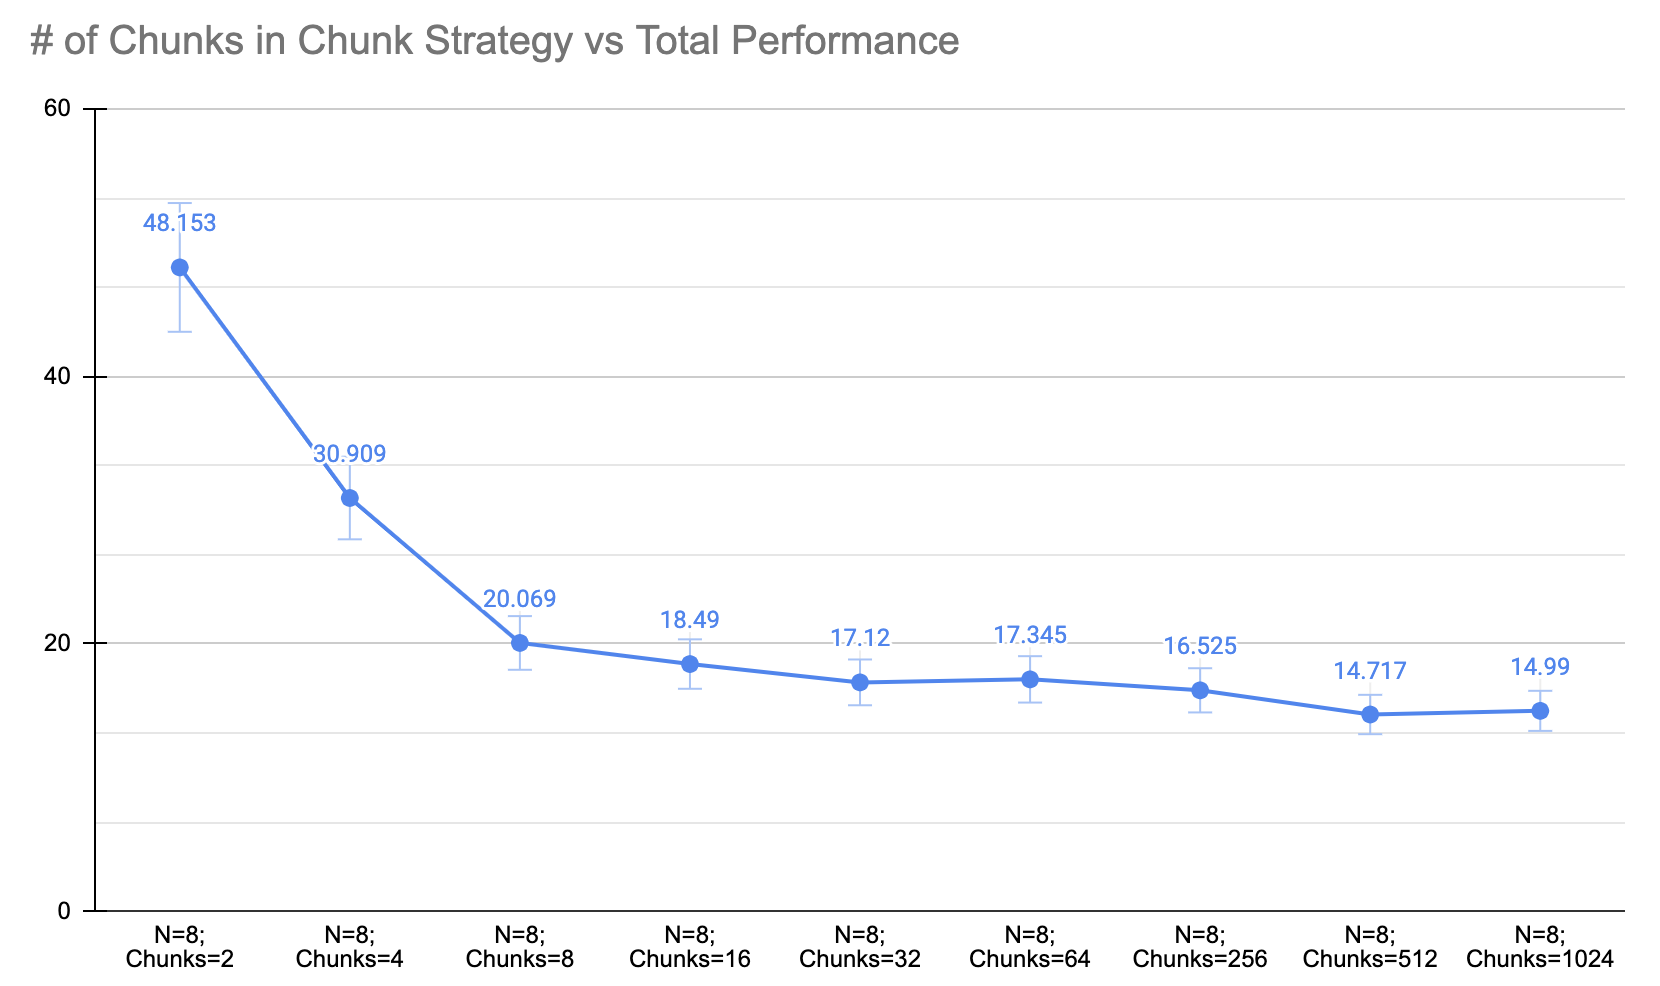
\includegraphics[width=40em]{../images/line_sc.png}
\end{figure}

It is also interesting to consider that on later turns, the possible solution set $P$ has shrunk. Thus, fewer chunks should be necessary for proper load balancing. An implementation was tested with various $n$ which split computation into $\frac{n}{2^k}$ chunks on turn $k$, however performance was not improved. Scaling factors of $1.2$ and $1.5$ were also tried. Again, there was no improvement over using the constant chunking.

% TODO do we need to discuss these shrinking chunk results quantitatively? -- Maybe not 

\section{Conclusion}
% TODO: maybe update if shrinking chunk was faster
To conclude, the chunked strategy was able to parallelize the Master Mind algorithm to run almost 3 times faster than the sequential version. We found that for our test setup, splitting computation at each turn into 512 chunks allowed for maximum performance. However, we suspect that the optimal number will differ based on the number of computational cores available. The game configuration (number of colors and holes) may also have an impact on determining how many chunks should be used. An interesting further investigation would be to have the algorithm adaptively determine how many chunks to use at each turn based on the game configuration, number of possible solutions remaining, and available hardware resources.

 % TODO bar graph showing best times from each method -- Solved
\begin{figure}[H]
	\centering
	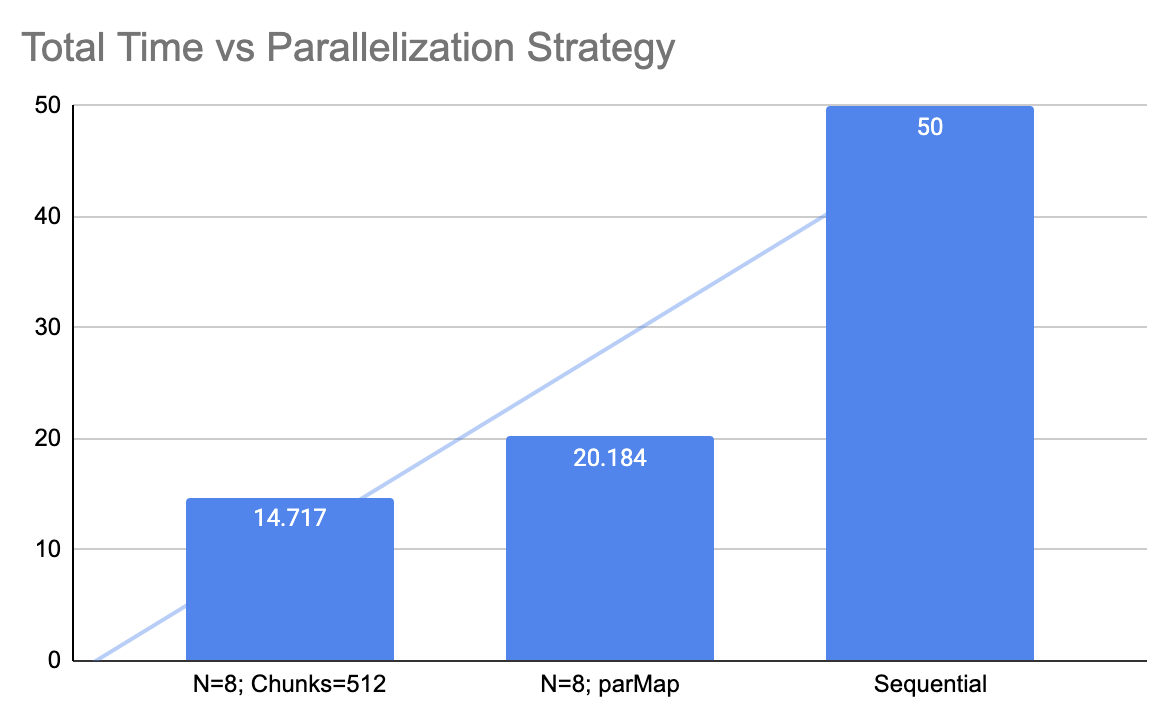
\includegraphics[width=40em]{../images/bar_sum.png}
\end{figure}


\section{Appendix: Code}
\label{sec:code}
%TODO: include all code files with minted -- Solved
\begin{minted}{haskell}
{-
 - Type Definition
-}
type ResponsePegs = (Int, Int) -- (#black, #white)

type Code = [Int]

type CodeSet = [Code]

type Possibility = (Int, Bool, Code) -- (Score, Invalid, Code)

{-
 - Utility Function
-}
parseCode :: String -> Code
parseCode str = (map read $ words str) :: [Int]

generateCodeSet :: (Eq a, Num a) => [a] -> a -> [[a]]
generateCodeSet [] _ = error "Give me a non-empty list"
generateCodeSet list hole
    | hole == 1           = [ [x] | x <- list]
    | otherwise           = [ x:xs | x <- list, xs <- generateCodeSet list $ hole - 1]
    
    
guessResult :: Code -> Code -> ResponsePegs
guessResult ans guess = (numBlack, numWhite)
    where numBlack = length $ filter id $ zipWith (==) ans guess
          numWhite = sum (map minCodeCount $ nub guess) - numBlack
          minCodeCount v = min (count v ans) (count v guess)
          count v ls = length $ filter (==v) ls


filterCodeSet :: CodeSet -> Code -> ResponsePegs -> CodeSet
filterCodeSet set guess response =
    filter ((response ==) . guessResult guess) set


scoreGuess :: CodeSet -> Code -> Possibility
scoreGuess possible code = (score, not valid, code)
    where
        valid = code `elem` possible
        allResponses = map (guessResult code) possible
        score = getMaxCount allResponses
        getMaxCount xs = foldl1' max $ map snd $ getCounts xs
        incCount o [] = [(o, 1)]
        incCount o (x@(v, c) : xs)
            | v == o = (v, c + 1) : xs
            | otherwise = x : incCount o xs
        getCounts xs = foldr incCount [] xs
       
      
splitToChunks :: Int -> [a] -> [[a]]
splitToChunks numChunks ls = chunk (length ls `quot` numChunks) ls
  where
    chunk _ [] = []
    chunk n ls = let (as, bs) = splitAt n ls in
      as : chunk n bs

bestFromChunk :: CodeSet -> CodeSet -> Possibility
bestFromChunk possibleSet chunk = foldl1' min $ map (scoreGuess possibleSet) chunk

{-
 - Main Function
-}
playMastermind ::  Code -> Code -> Int -> CodeSet -> CodeSet -> IO Int
playMastermind guess solution k fullSet possibleSet = do
  putStrLn $ "Guessing: " ++ show guess
  let response@(blk, wht) = guessResult guess solution
  putStrLn $
    "Response: " ++ show blk ++ " black and "
      ++ show wht ++ " white"
  if blk == length guess then do
    putStrLn $ "Solved: " ++ show guess
    return k
  else do
    let possibleSet' = filterCodeSet possibleSet guess response
    let possibilities = map (scoreGuess possibleSet') fullSet
    let (_, _, nextGuess) = minimum possibilities
    playMastermind nextGuess solution (k + 1) fullSet possibleSet'



playMastermindParMap ::  Code -> Code -> Int -> CodeSet -> CodeSet -> IO Int
playMastermindParMap guess solution k fullSet possibleSet = do
  putStrLn $ "Guessing: " ++ show guess
  let response@(blk, wht) = guessResult guess solution
  putStrLn $
    "Response: " ++ show blk ++ " black and "
      ++ show wht ++ " white"
  if blk == length guess then do
    putStrLn $ "Solved: " ++ show guess
    return k
  else do
    let possibleSet' = filterCodeSet possibleSet guess response
    let possibilities = runPar $ parMap (scoreGuess possibleSet') fullSet
    let (_, _, nextGuess) = minimum possibilities
    playMastermindParMap nextGuess solution (k + 1) fullSet possibleSet'
    
  
playMastermindChunkStrategy ::  Int -> Code -> Code -> Int -> CodeSet -> CodeSet -> IO Int
playMastermindChunkStrategy numChunks guess solution k fullSet possibleSet = do
  putStrLn $ "Guessing: " ++ show guess
  let response@(blk, wht) = guessResult guess solution
  putStrLn $
    "Response: " ++ show blk ++ " black and "
      ++ show wht ++ " white"
  if blk == length guess then do
    putStrLn $ "Solved: " ++ show guess
    return k
  else do
    let possibleSet' = filterCodeSet possibleSet guess response
    let chunks = splitToChunks numChunks fullSet -- TODO: Tune the number of chunks
    let possibilities = map (bestFromChunk possibleSet') chunks `using` parList rseq
    let (_, _, nextGuess) = foldl1' min possibilities
    playMastermindChunkStrategy numChunks nextGuess solution (k + 1) fullSet possibleSet'



{-
 - Entry Function @ app/Main.hs
-}
readInt :: IO Int
readInt = readLn

main :: IO ()
main = do
    putStrLn "Game Configuration: How many colors?"
    numColors <- readInt
    putStrLn "Game Configuration: How many holes?"
    numHoles <- readInt
    putStrLn $
        "Config: " ++ show (numColors :: Int) ++ " colors and "
        ++ show (numHoles :: Int)
        ++ " holes"
    putStrLn "What is the solution code?"
    solStr <- getLine
    let sol = parseCode solStr
    if (length sol /= numHoles)
        || isJust (find (\x -> x > numColors || x < 0) sol) then 
            putStrLn "Invalid input code!"
    else do
        let initialGuess = replicate numHoles 1 
        let codeset = generateCodeSet [1 .. numColors] numHoles
        num_turns_required <- playMastermindChunkStrategy 512 initialGuess sol 1 codeset codeset
        putStrLn $ "Solved in " ++ show num_turns_required ++ " turns"
\end{minted}

\section{Appendix: Dependencies, Compiler Options, and Executable Options}
\begin{minted}{yaml}
    dependencies: 
    - master-minds
    - monad-par >= 0.3.5
    - parallel >= 3.2.2.0
\end{minted}

\begin{minted}{yaml}
    ghc-options:
    - -O2
    - -threaded
    - -rtsopts
    - -eventlog
\end{minted}

\begin{minted}{bash}
    ./master-minds -f +RTS -N8 -ls -s <<-EOF
    10
    4
    8 7 6 5
    EOF
\end{minted}



\end{document}
